\documentclass[10pt,a4paper]{article}
\usepackage[utf8]{inputenc}
\usepackage{amsmath}
\usepackage{graphicx}
\usepackage{subfigure}
\usepackage{subfig}
\usepackage{amsfonts}
\usepackage{float}
\setlength{\parindent}{0cm}
\usepackage{amssymb}
\author{Ferreyra Emanuel, Martin Rafael, Postolski Ivan}
\title{Modelado y simulación para un sistema controlado de din\'amica SIR con Vacunación en un entorno de grafo estoc\'astico.}




\begin{document}

%%%% PROCESAR con PdfLaTeX !!!!!


%\documentclass[12pt]{book}
%\usepackage{geometry}\geometry{top=5cm,bottom=2cm,left=3cm,right=3cm}
%\usepackage{amssymb}
%\usepackage{amsmath}
%\usepackage{graphicx}
%\usepackage{txfonts}




%\begin{document}
\thispagestyle{empty}

\begin {center}


\includegraphics[scale=.3]{uba2.jpg}

\medskip
\textbf{UNIVERSIDAD DE BUENOS AIRES}

\smallskip

\textbf{Facultad de Ciencias Exactas y Naturales}

\smallskip

\textbf{Departamento de Computaci\'on}

\vspace{3.5cm}

\textbf{\large Simulaci\'on de Eventos Discretos 2017}


\vspace{3cm}

\vspace{1.5cm}

\textbf{\large TP2: Modelo FHP para un aut\'omata celular de gas en reticulado.}

\vspace{1.5cm}


\textbf{Ferreyra Emanuel; Martin Rafael; Postolski Ivan}

\end {center}


\vspace{1.5cm}

\noindent \textbf{Profesor: Rodrigo Castro} \




%\end{document}


\bigskip


\part*{Modelo Conceptual}
Las ecuaciones de Navier-Stokes reciben su nombre de Claude-Louis Navier y George Gabriel Stokes. Se trata de un conjunto de ecuaciones en derivadas parciales no lineales que describen el movimiento de un fluido. Estas ecuaciones gobiernan la atm\'osfera terrestre, las corrientes oce\'anicas y el flujo alrededor de veh\'iculos o proyectiles y, en general, cualquier fen\'omeno en el que se involucren fluidos newtonianos. 

\begin{figure}[H]
\centering
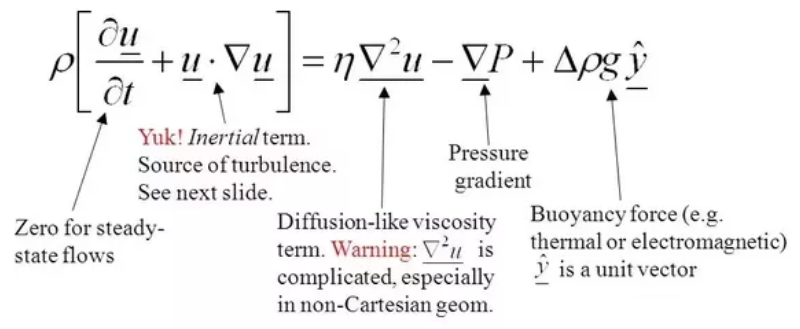
\includegraphics[scale=0.4]{NS}
\caption{Ecuaciones de Navier-Stokes}
\end{figure}

No se dispone de una soluci\'on general para este conjunto de ecuaciones, y salvo ciertos tipos de flujo y situaciones muy concretas no es posible hallar una soluci\'on anal\'itica. Por lo que en muchas ocasiones es preciso recurrir al an\'alisis numérico para determinar una soluci\'on aproximada.

En 1986 Uriel Frisch, Brosl Hasslacher y Yves Pomeau propusieron un modelo (FHP) de ``lattice gas'' equivalente a resolver las ecuaciones de Navier-Stokes.

\begin{figure}[H]
\centering
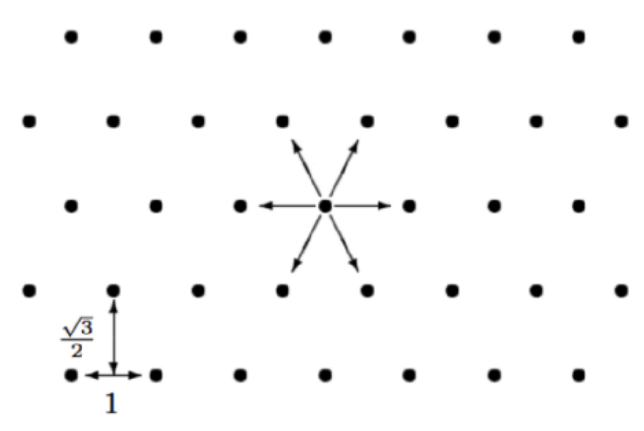
\includegraphics[scale=0.4]{grilla}
\caption{grilla hexagonal propuesta por FHP}
\end{figure}

La din\'amica tendr\'a las siguientes propiedades:
\begin{enumerate}
\item Cada nodo es una celda hexagonal,
\item Cada nodo puede o no tener una part\'icula,
\item Cada part\'icula tiene una direcci\'on de movimiento.
\end{enumerate}

En cada paso de la simulaci\'on se deben respetar dos invariantes:

\begin{enumerate}
\item La cantidad de part\'iculas no cambia.
\item El momento se mantiene constante.
\end{enumerate}

Para ello las reglas de resoluci\'on de choques deben ser consecuentes con estos invariantes.

\begin{figure}[H]
\centering
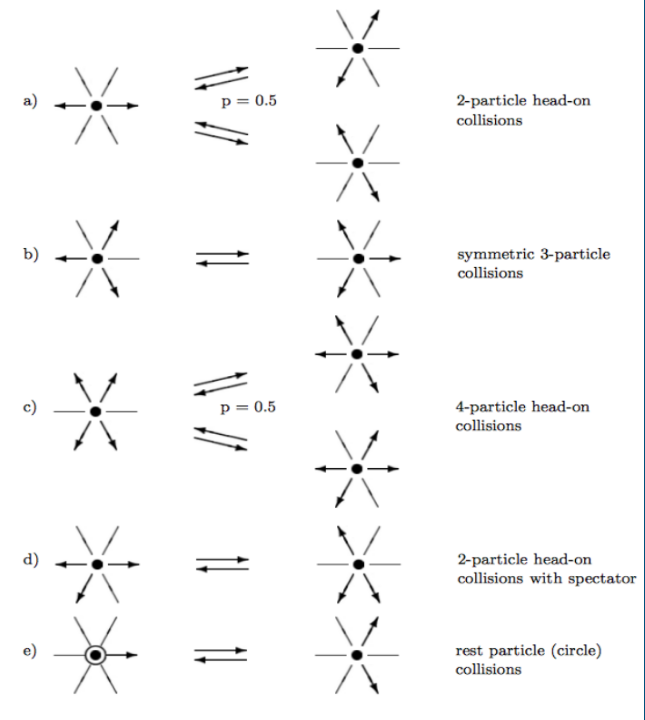
\includegraphics[scale=0.4]{colisiones}
\caption{Ejemplos de resoluci\'on de choque para algunas particulas}
\end{figure}

El objetivo del trabajo es implementar este modelo en Cell-Devs y simular algunos casos sencillos, principalmente el de un fluido ``viajando'' por un caño con obstrucciones.

\section*{Dificultades, Simplificaciones y Modelado}
La primer simplificaci\'on del modelo fue la reducci\'on de las colisiones a analizar. Las dificultades para manejar eventos simult\'aneos en Cell-DEVS generaban incoventientes en identificar como resolver los choques para actualizar las posiciones de las part\'iculas puesto que cada una de ellas debe observar a toda su vecindad y esta estar sincronizada para poder actualizar el valor.

Por esto es que decidimos que el gas tuviera una direccionalidad limitando a tres las posibles velocidades de las part\'iculas (derecha, arriba-derecha, abajo-derecha). Haciendo esto reducimos la resoluci\'on de choques a propagar el gas en la direcci\'on que llevaba, como si estuviera en un ca\~no. En esto, simplemente hay que tener cuidado con los l\'imites superior e inferior.

Es importante aclarar, que teniendo este supuesto, todas las celdas se comportan de la misma manera, ya sean de filas pares o impares, algo que en realidad no sucede en este tipo de modelos hexagonales.

\begin{figure}[H]
\centering
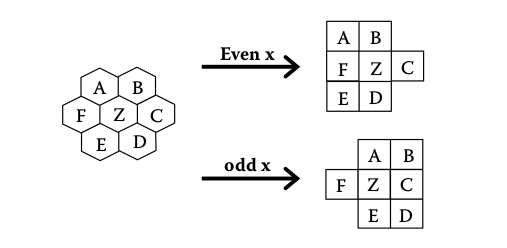
\includegraphics[scale=0.4]{vecindad}
\caption{Vecindades hexagonales}
\end{figure}

Como el gas se mueve solo en una direcci\'on (a la derecha), cada celda debe mirar que hay en sus tres vecinos de la izquierda para actualizarse, comport\'andose todas como si pertenecieran a filas pares.

Con el fin de que dicha actualizaci\'on se realice con las celdas sincronizadas es que el valor de cada c\'elula es una tupla que contiene la direcci\'on en la que se est\'a propagando el gas y el paso temporal en el que esto sucede. Esto lo hacemos v\'ia los macros \textit{AdelanteSincronizado}, \textit{AdelanteSincronizadoMasUno} y \textit{AtrasSincronizado}.

Para las direcciones utilizamos una codificaci\'on basada en la escritura \'unica en base 2. La direcci\'on arriba a la derecha representada por $2^0$, a la derecha por $2^1$ y abajo a la derecha por $2^2$. As\'i, el valor $5=2^0+2^2$ en una celda representa que hay dos part\'iculas, una moviendose hacia arriba y la otra hacia abajo (ambas hacia la derecha).

Con esta idea, los valores para identificar los bordes son 8 y 16 para los correspondientes superior e inferior. En los casos que la part\'icula se dirija hacia un borde, \'esta rebotar\'a con direcci\'on opuesta, lo cual es una excepci\'on a la
invarianza del momento. Utilizamos macros para chequear estas condiciones y obtener el comportamiento deseado.

Las dos limitaciones de nuestra implementaci\'on que terminaron siendo las m\'as restrictivas con respecto a los experimentos que quer\'iamos hacer fueron que las part\'iculas no puedan volver y que no podamos tener dos part\'iculas en la misma celda moviendose en la misma direcci\'on.


\section*{Testing}

%Para testear que las interacciones se sucedieran como era esperado trabajamos con cuadr\'iculas con bordes superior e inferior colocando en el extremo izquierdo de esta una columna de datos iniciales diferentes cada vez, y chequeando que la columna de gas se moviera hacia la derecha resolviendo correctamente las colisiones y manteniendo cada part\'icula la direcci\'on adecuada. 

\subsection*{Trump wall}
\textbf{Configuración inicial}: Colocar en los bordes superiores e inferiores valores correspondientes a paredes y ningún otro valor en otras celdas.


\textbf{Configuración esperada}: Que nada cambie.

\subsection*{Forrest Gump}
\textbf{Configuración inicial}: Ubicar una sola partícula con dirección hacia la derecha (2) en el borde izquierdo.

\textbf{Configuración esperada}: Que la partícula solo se desplace hacia la derecha.

\subsection*{Zombies}
\textbf{Configuración inicial}: Ubicar una columna inicial a la izquierda de partículas con dirección hacia la derecha. 


\textbf{Configuración esperada}: Que la columna avance toda junta hacia la derecha.

\subsection*{Pong}
\textbf{Configuración inicial}: Setear bordes inferiores y superiores, luego ubicar una partícula con dirección diagonal (1 o 4) en el borde izquierdo.  

\textbf{Configuración esperada}: Que los choques con las paredes se realicen adecuadamente, o sea, pasar de un 1 a un 4 y viceversa.

\subsection*{Gotenks}
\textbf{Configuración inicial}: Inicializar con dos partículas destinadas a chocar.


\textbf{Configuración esperada}: Que el choque se realice apropiadamente, conservando el momento y la cantidad de partículas.

\subsection*{Home alone}
\textbf{Configuración inicial}: Bordes superiores e inferiores con flujo inicial variable.


\textbf{Configuración esperada}: Que al terminar la simulación la cantidad de partículas siga siendo la misma.

\paragraph{}
Todos los comportamientos de la versión entregada se correspondieron con los esperados en los tests, validando los casos considerados interesantes.

 

\part*{Experimentaci\'on mediante Simulaci\'on}
\section*{Resultados de la simulaci\'on}

Entre los experimentos que plane\'abamos hacer se encontraban analizar como evolucionaba el gas en un tubo angost\'andose, o c\'omo interactuaba con otras part\'iculas solidas fijas dispuestas en el medio del ambiente, o un modelo del tipo Ehrenfest (que por estar te\'oricamente resuelto ser\'ia id\'oneo para validar). La realidad es que la limitaci\'on de no poder modelar dos part\'iculas en la misma posici\'on movi\'endose en la misma direcci\'on hizo que estas tres situaciones estuvieran fuera de nuestro alcance.

La experimentaci\'on que pudimos llevar a cabo satisfactoriamente fue la de considerar separaciones horizontales entre dos sectores por los que se mueve gas y, eventualmente, eliminar dicha separaci\'on. Con esto el espacio en el que se mueve el gas se ve repentinamente m\'as grande y part\'iculas de los dos sectores comienzan a interactuar.

\begin{figure}[htbp]
\centering
\subfigure[Estado inicial]{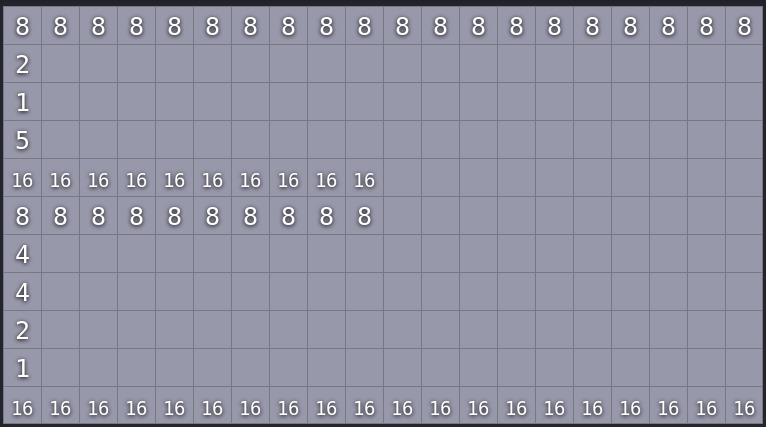
\includegraphics[width=40mm]{1.jpeg}}
\subfigure[Estado intermedio]{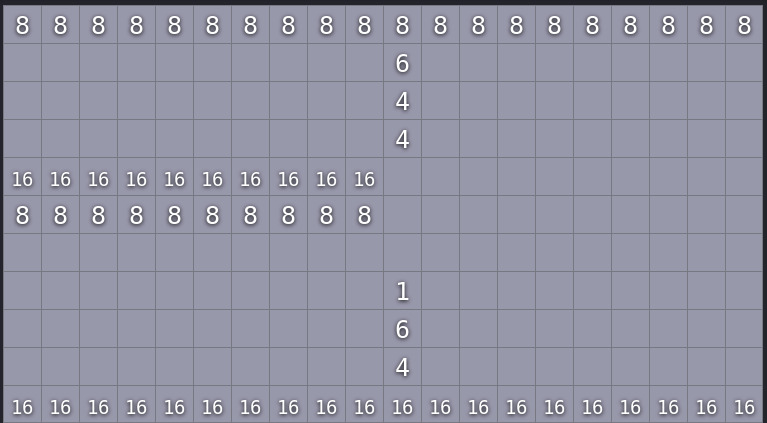
\includegraphics[width=40mm]{2.jpeg}}
\subfigure[Estado final]{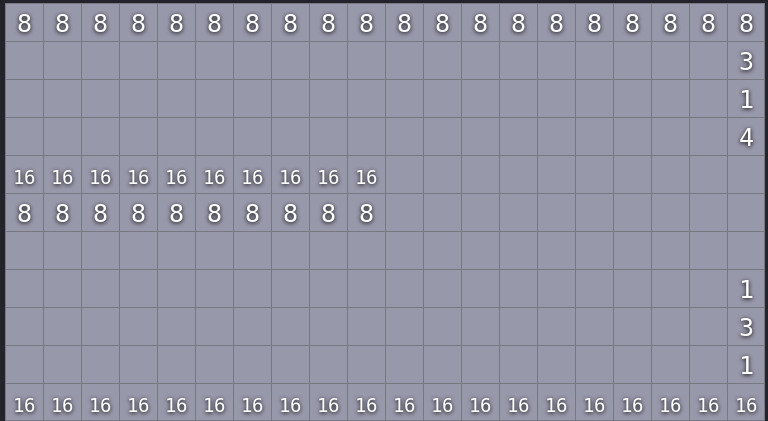
\includegraphics[width=40mm]{3.jpeg}}
\caption{Ejemplo evoluci\'on simulaci\'on}
\end{figure}



Este modelo es un comienzo para algo que a futuro podr\'a desarrollarse mejor, incorpor\'ando reglas y restricciones para darle m\'as direccionalidad al movimiento de las part\'iculas de gas.



\end{document}



